\chapter{Resultados}\label{cap:resultados}

Esta pesquisa explora a transferência de aprendizado utilizando modelos pré-treinados no dataset ImageNet, aplicando ajuste fino para classificar o nível de severidade da osteoartrite de joelho com base na escala de Kellgren/Lawrence. O treinamento dos modelos foi realizado com a linguagem de programação Python, através de notebooks disponibilizados pela plataforma Google Colab, aproveitando os recursos computacionais de uma GPU T4 para acelerar o treino e a experimentação.

A classificação da osteoartrite de joelho foi organizada em quatro cenários: (i) classificação com 5 classes, (ii) classificação com 4 classes, (iii) classificação com 3 classes e (iv) classificação binária. O primeiro cenário foi o mais complexo, pois envolveu a classificação em cinco classes distintas (KL0, KL1, KL2, KL3 e KL4), enquanto os outros cenários foram simplificações do primeiro, reduzindo o número de classes a serem classificadas. A escolha do cenário de cinco classes foi motivada pela necessidade de uma classificação mais detalhada e precisa da osteoartrite de joelho, permitindo uma melhor avaliação da progressão da doença.

Para garantir a consistência entre os modelos, o treinamento foi realizado utilizando os mesmos hiperparâmetros. O conjunto de dados foi dividido em 70\% para treinamento, 10\% para teste e 20\% para validação. Para mitigar possíveis vieses, a base de dados foi balanceada por meio de técnicas de \textit{undersampling} e \textit{oversampling}, limitando cada classe a um máximo de 1700 imagens, complementadas por estratégias de \textit{data augmentation}. O treinamento foi configurado com \textit{batches} de 28 imagens, executado ao longo de 30 épocas, com um \textit{early stopping} com 5 épocas de paciência para evitar \textit{overfitting}.

Neste estudo, foi utilizada duas abordagens de função de perda: \textit{crossentropy} e \textit{CORN} (Conditional Ordinal Regression for Neural Networks). A função de perda \textit{crossentropy} é amplamente utilizada em tarefas de classificação, enquanto a função de perda CORN é projetada especificamente para problemas de classificação ordinal, onde a ordem das classes é relevante. Essa abordagem é particularmente útil em cenários onde as classes não são mutuamente exclusivas, como na classificação da osteoartrite de joelho, onde os estágios da doença são sequenciais e possuem uma relação ordinal. Em ambos os casos, o otimizador adotado foi o Adam, configurado com uma taxa de aprendizado inicial de 0.0001, ajustada dinamicamente a cada 3 épocas.

\subsection{Classificação em Cinco Classes}

A \autoref{label:resultados-5-crossentropy} apresenta os resultados dos modelos de RNCs e ViTs treinados para a classificação da OA de joelho usando a função de perda \textit{crossentropy}. A acurácia geral dos modelos variou de 0.6922 a 0.7363, com o modelo GCViT apresentando a maior acurácia geral de 0.7363. Além disso, o modelo GCViT também obteve o melhor desempenho em termos de Kappa, QWK e MAE, com valores de 0.6372, 0.8725 e 0.2940, respectivamente. Esses resultados indicam que o modelo GCViT foi capaz de aprender padrões relevantes para a classificação da OA de joelho, superando os demais modelos avaliados.

O modelo DaViT também apresentou um desempenho notável, com uma acurácia geral de 0.7358, Kappa de 0.6362, QWK de 0.8647 e MAE de 0.3023. Esses resultados sugerem que o modelo DaViT é eficaz na extração de características relevantes em imagens médicas, embora tenha apresentado um desempenho ligeiramente inferior ao do modelo GCViT.

A \autoref{tab:resultados} mostra a acurácia dos modelos de RNCs e ViTs treinados para a classificação da OA de joelho usando a função de perda \textit{crossentropy}. Em relação ao tempo de treinamento, é possível notar que o modelo mais rápido foi o ResNet-50, com um tempo de 11.29 segundos. Por outro lado, o modelo mais lento foi o DeiT, com um tempo de 79.5 segundos. Tais valores não necessariamente indicam que o modelo mais rápido é o pior, ou o contrário, mas é importante considerar o tempo de treinamento como um fator relevante ao escolher um modelo, especialmente se houver restrições de recursos computacionais. O tempo de treinamento mostrado varia, principalmente, com o número de épocas, já que modelos que levaram mais tempo são aqueles que tiveram a parada antecipada mais tarde, ou executaram as 30 épocas completas.
'
\begin{table}
    \centering
    \caption{Desempenho dos modelos utilizando a abordagem Cross Entropy}
    \begin{tabular}{lcccc}
        \toprule
        \textbf{Modelo} & \textbf{Accuracy} & \textbf{Kappa} & \textbf{QWK} & \textbf{MAE} \\
        \midrule
        resnet34       & 0.7027 & 0.5899 & 0.8422 & 0.3469 \\
        resnet50       & 0.7104 & 0.6014 & 0.8478 & 0.3354 \\
        resnet101      & 0.6961 & 0.5800 & 0.8406 & 0.3541 \\
        vgg16          & 0.6922 & 0.5691 & 0.8290 & 0.3696 \\
        vgg19          & 0.7060 & 0.5888 & 0.8404 & 0.3497 \\
        densenet121    & 0.7204 & 0.6110 & 0.8514 & 0.3271 \\
        densenet169    & 0.7220 & 0.6158 & 0.8519 & 0.3249 \\
        inception\_v3  & 0.7022 & 0.5931 & 0.8500 & 0.3376 \\
        google\_vit    & 0.7005 & 0.5878 & 0.8380 & 0.3497 \\
        facebook\_deit & 0.6939 & 0.5775 & 0.8342 & 0.3585 \\
        davit          & 0.7358 & 0.6362 & 0.8647 & 0.3023 \\
        maxvit\_t      & 0.7220 & 0.6165 & 0.8616 & 0.3155 \\
        gcvit          & \textbf{0.7363} & \textbf{0.6372} & \textbf{0.8725} & \textbf{0.2940} \\
        swin\_b        & 0.6977 & 0.5805 & 0.8425 & 0.3508 \\
        \bottomrule
    \end{tabular}
    \label{tab:resultados-5-crossentropy}
\end{table}

Quanto à acurácia geral (\textit{overall}), todos os modelos apresentaram resultados razoavelmente bons, com valores variando de 0.6723 a 0.7319. Isso indica que todos os modelos foram capazes de aprender padrões relevantes para a classificação da OA de joelho. No entanto, é importante notar que o modelo DenseNet-169 obteve a maior acurácia geral, com um valor de 0.7319. Isso sugere que arquiteturas de RNCs densamente conectadas podem ser muito eficazes na extração de características relevantes em imagens médicas como radiografias de joelho. Além disso, os modelos de conexões residuais (ResNet) também apresentaram resultados competitivos, com acurácias gerais variando de 0.7044 a 0.7248, onde o ResNet-50 obteve a maior acurácia dentre eles e com o menor tempo de treinamento, oferecendo um bom equilíbrio entre generalização do modelo e custo computacional.

Por outro lado, os modelos da família VGG (VGG-16 e VGG-19) apresentaram acurácias gerais mais baixas, variando de 0.6723 a 0.6851, o que sugere que essas arquiteturas mais simples podem não ser tão eficazes na extração de características complexas em radiografias de joelho. Embora fosse esperado que esses modelos tivessem desempenho inferior em relação aos modelos ResNet, devido à sua profundidade, os resultados indicam que esses modelos são capazes de aprender padrões relevantes e ter uma menor probabilidade de \textit{overfitting}, como observado no tempo de treinamento do VGG-16, que foi maior que a maioria dos modelos justamente por não ter parada antecipada em virtude da queda do erro no conjunto de validação.

O GoogLeNet, com sua arquitetura Inception (versão 3), permitiu que o modelo tivesse uma acurácia geral de 0.7215, indicando que o modelo pode ser eficaz na extração de características relevantes e superar a maioria dos modelos de RNCs. Esse comportamento pode ser justificado pelo uso de uma técnica chamada de "bottleneck" ou "redução de dimensionalidade", que reduz a quantidade de parâmetros e a complexidade computacional do modelo, sem comprometer significativamente o desempenho.

Os modelos de transformers, por sua vez, apresentaram acurácias gerais variando de 0.6862 a 0.7215, indicando que essas arquiteturas podem ser eficazes, mas talvez não sejam tão eficientes quanto os modelos de RNCs. O modelo Swin Transformer obteve a maior acurácia geral entre os modelos de transformers, com um valor de 0.6977, sugerindo que a abordagem hierárquica de atenção pode ser eficaz na extração de características relevantes em radiografias de joelho.

Entretanto, é importante notar que a acurácia para a classe KL 1 foi baixa para todos os modelos, variando de 0.2562 e 0.4475. Isso indica que a classificação da OA de joelho no estágio 1 (duvidoso) pode ser mais desafiadora, possivelmente devido à semelhança visual com as classes adjacentes KL 0 e KL 2. Esse resultado pode ser observado na \autoref{confusion-matrix-resnet50}, que mostra a matriz de confusão do modelo ResNet-50. A classe KL 1 tem a menor acurácia dentre todas as classes, o que reflete o desafio na classificação dessa classe devido ao nível de detalhe ou até mesmo incoerência no rotulação das imagens do dataset.

\begin{figure}[h]
    \centering
    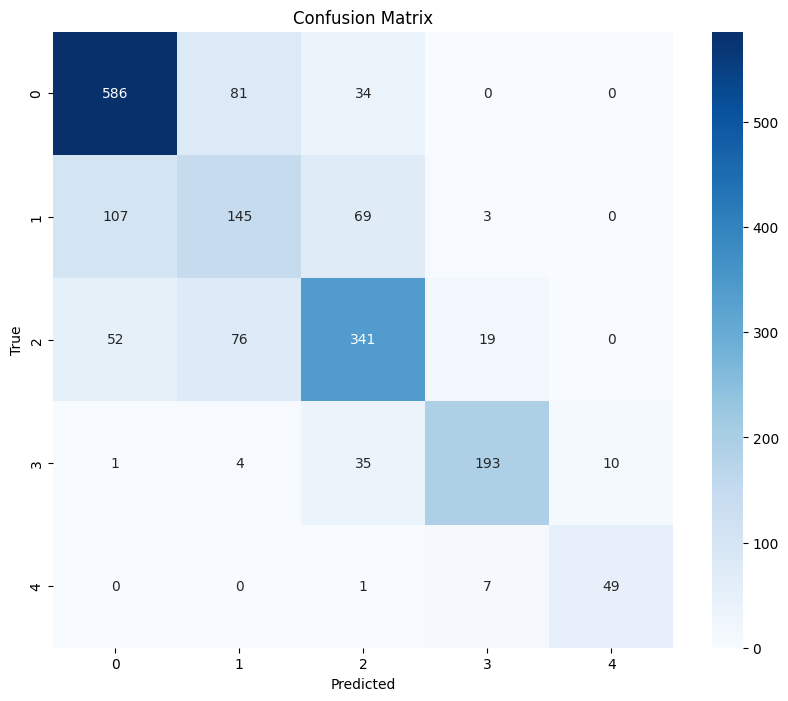
\includegraphics[width=\linewidth]{figs/confusion-matrix-resnet50.png}
    \caption{Matriz de confusão do modelo ResNet-50.}
    \label{confusion-matrix-resnet50}
\end{figure}

Em resumo, os modelos ResNet-50 e DenseNet-169 se destacaram em termos de tempo de treinamento e acurácia geral, respectivamente. No entanto, é importante considerar as características de cada classe ao escolher um modelo, pois diferentes modelos podem ter desempenhos diferentes para cada classe.

A \autoref{tab:resultados-corn} apresenta os resultados dos modelos de RNCs e ViTs treinados para a classificação da OA de joelho usando a função de perda CORN. Em relação ao tempo de treinamento, não houve uma mudança significativa comparado com a função de perda \textit{crossentropy}. O modelo mais rápido foi, novamente, o ResNet-50, com um tempo de 10.32 segundos, enquanto o modelo mais lento foi o Swin Transformer, com um tempo de 35.58 segundos. Em relação à acurácia geral, os resultados variaram de 0.6546 a 0.7181, indicando que a função de perda CORN pode ser eficaz na classificação da OA de joelho, mas não necessariamente supera a função de perda \textit{crossentropy}. Isso é justificado pelo fato de que a função de perda CORN é mais adequada quando o modelo faz predições mais afastadas do rótulo real, o que não foi evidenciado ao observar as matrizes de confusão dos modelos.

\begin{table}
    \centering
    \begin{tabular}{|c|c|c|c|c|c|c|c|}
        \hline
        \multirow{2}{*}{Modelo} & \multirow{2}{*}{Tempo} & \multirow{2}{*}{Overall} & \multicolumn{5}{|c|}{Classe KL} \\ \cline{4-8}
        &  &  & 0 & 1 & 2 & 3 & 4 \\ \hline
        ResNet-34 & 14.93 & 0.6895 & 0.7518 & 0.5586 & 0.6107 & 0.8107 & 0.8246 \\ \hline
        ResNet-50 & 10.32 & 0.7181 & 0.796 & 0.5031 & 0.6824 & 0.823 & 0.8421 \\ \hline
        ResNet-101 & 16.17 & 0.6994 & 0.7418 & 0.4506 & 0.707 & 0.8519 & 0.8772 \\ \hline
        VGG-16 & 19.29 & 0.6762 & 0.7646 & 0.358 & 0.6824 & 0.7984 & 0.8246 \\ \hline
        VGG-19 & 24.05 & 0.6669 & 0.7974 & 0.3549 & 0.6066 & 0.7901 & 0.8246 \\ \hline
        DenseNet-121 & 10.62 & 0.6911 & 0.729 & 0.4444 & 0.7172 & 0.8272 & 0.8246 \\ \hline
        DenseNet-169 & 13.75 & 0.717 & 0.7874 & 0.5833 & 0.6393 & 0.8148 & 0.8596 \\ \hline
        Inception-v3 & 17.09 & 0.701 & 0.7932 & 0.5093 & 0.6639 & 0.7325 & 0.8421 \\ \hline
        ViT-B & 36.97 & 0.6817 & 0.7447 & 0.4815 & 0.6393 & 0.8066 & 0.8772 \\ \hline
        DeiT & 34.73 & 0.6602 & 0.7047 & 0.4877 & 0.6209 & 0.7984 & 0.8421 \\ \hline
        Swin & 35.58 & 0.6546 & 0.7803 & 0.4658 & 0.6722 & 0.8395 & 0.7894 \\ \hline
    \end{tabular}
    \caption{Desempenho dos modelos de RNCs e ViTs na classificação da OA de joelho usando a função da perda CORN.}
    \label{tab:resultados-corn}
    \end{table}

No entanto, é importante notar que o modelo ResNet-50 obteve a maior acurácia geral, com um valor de 0.7181, superando os demais modelos, inclusive o modelo DenseNet-169, que obteve a maior acurácia geral com a função de perda \textit{crossentropy}. Isso sugere que a função de perda CORN pode ser eficaz em arquiteturas de RNCs, especialmente aquelas com conexões residuais. Entretanto, o modelo DenseNet-169 foi quem obteve a maior acurácia para a classe KL 1, com um valor de 0.5833, que é a classe mais desafiadora de ser classificada, como observado anteriormente.

\section{Resultados e Discussão}

\subsection{Visão Geral dos Resultados}

Os experimentos envolveram avaliação de 18 arquiteturas (CNN e ViT), cada uma treinada com duas funções de perda: \emph{cross entropy} e \emph{Corn} (cumulative ordinal regression). As métricas principais consideradas foram acurácia, kappa de Cohen (coeficiente de concordância), weighted Quadratic Weighted Kappa (QWK) e Mean Absolute Error (MAE). A Tabela~\ref{tab:resultados} resume os cinco modelos com melhor desempenho em termos de QWK, para ambas as funções de perda.

\subsection{Discussão}

Observa-se que o modelo \textbf{GCViT} apresentou o melhor desempenho global, atingindo QWK de 0.8725 com \emph{cross entropy} e 0.8752 com \emph{Corn}, além de MAE mínimo de 0.29399 e 0.29123, respectivamente;:contentReference[oaicite:1]{index=1}. Logo em seguida, os modelos \textbf{DaViT} e \textbf{MaxViT\_T} também se destacaram, com QWK acima de 0.86 e MAE abaixo de 0.32, evidenciando a eficácia de transformers especializados para tarefas de classificação ordinal de osteoartrite.

Entre as CNNs, as versões densas (\emph{DenseNet169} e \emph{DenseNet121}) obtiveram desempenhos notáveis, com QWK acima de 0.85 e acurácias próximas a 72\% sob \emph{cross entropy}, mas ficaram abaixo dos ViTs em QWK e MAE;:contentReference[oaicite:3]{index=3}.

Ainda, a função de perda \emph{Corn} mostrou ligeira melhora em QWK para a maioria dos modelos de ViT, embora com tempo de treinamento tipicamente maior do que com \emph{cross entropy} (por exemplo, GCViT: 3454\,s vs.\ 2423\,s);:contentReference[oaicite:5]{index=5}.

\begin{table}[htb]
\centering
\caption{Desempenho dos cinco melhores modelos (ordem por QWK) para as duas funções de perda.}
\label{tab:resultados}
\begin{tabular}{l|ccccc|ccccc}
\hline
\multirow{2}{*}{\textbf{Modelo}} & \multicolumn{5}{c|}{\textbf{Cross Entropy}} & \multicolumn{5}{c}{\textbf{Corn}} \\
 & Acc. & Kappa & QWK & MAE & Tempo (s) & Acc. & Kappa & QWK & MAE & Tempo (s) \\
\hline
GCViT        & 0.7363 & 0.6372 & 0.8725 & 0.29399 & 3454.0 & 0.7347 & 0.6369 & 0.8752 & 0.29123 & 2422.6 \\
DaViT        & 0.7358 & 0.6362 & 0.8647 & 0.30226 & 3045.0 & 0.7286 & 0.6288 & 0.8713 & 0.29950 & 2342.1 \\
MaxViT\_T    & 0.7220 & 0.6165 & 0.8616 & 0.31550 & 1489.6 & 0.7038 & 0.5934 & 0.8636 & 0.32267 & 1006.4 \\
DenseNet169  & 0.7220 & 0.6158 & 0.8519 & 0.32488 &  888.2 & 0.7187 & 0.6143 & 0.8660 & 0.31219 & 1345.6 \\
DenseNet121  & 0.7204 & 0.6110 & 0.8514 & 0.32708 & 1148.4 & 0.7071 & 0.6001 & 0.8592 & 0.32377 &  624.8 \\
\hline
\end{tabular}
\end{table}

\subsection{Principais Conclusões}

\begin{itemize}
  \item \textbf{GCViT} foi o modelo de melhor desempenho, com QWK máximo de 0.8752 (Corn) e MAE mínimo de 0.2912, indicando superior capacidade de modelar a natureza ordinal da escala KL.
  \item Transformers (GCViT, DaViT, MaxViT\_T) superaram consistentemente as CNNs clássicas em QWK e MAE, embora demandem maior custo computacional.
  \item A função de perda \emph{Corn} proporcionou ganhos moderados em QWK para ViTs, justificando seu uso em tarefas de classificação ordinal.
  \item Dentre as CNNs, \emph{DenseNet169} e \emph{DenseNet121} foram as mais competitivas, alcançando QWK acima de 0.85.
\end{itemize}
